\chapter{Introducción}

En este capítulo se explicará el concepto de robótica móvil\cite{RoboticaMovil}.
También se comentarán los robots submarinos, ya que en este proyecto, trataremos sobre uno de ellos, OpenROV.
Hablaremos sobre ROS (Robot Operating System), que tiene un conjunto de herramientas y atajos que facilitan la comunicación y operabilidad de los robots porque en uno de los capítulos del proyecto, se expondrá la integración de este framework en el ROV.
El estado del arte y la estructura de la memoria son los otros dos puntos que se tratarán en éste capítulo.

\section{Robótica móvil}
\label{cap:roboticamovil}
Generalmente las aplicaciones robóticas se centraban en los sectores manufactureros más desarrollados para la producción masiva: industria del automóvil, transformaciones metálicas, etc.

A principios de los años sesenta se introducen en la industria los robots manipuladores como un elemento más del proceso productivo. Los trabajos desarrollados por los robots manipuladores consistían frecuentemente en tareas repetitivas.

Un robot móvil puede moverse sobre entornos no estructurados, de los cuales, no se posee conocimiento. Esto lo realiza mediante la interpretación de los datos obtenidos a través de los sensores y del estado actual del vehículo. 

En general se considera que existen tres clases de robots:
\begin{itemize}
\item \textbf{Industriales} son los de mayor difusión en tareas de alcance económico, formados por una estructura mecánica articulada, que se mueve adoptando distintas configuraciones por las órdenes recibidas de un equipo de control basado normalmente en un microprocesador.
\item \textbf{Medicos}  de cooperación o de rehabilitación están concebidos como prótesis inteligentes para los disminuidos físicos. Se procura que tenga la estética correspondiente a la extremidad humana.
\item \textbf{Móviles} tienen una plataforma mecánica dotada de un sistema de locomoción capaz de navegar a través de un determinado ambiente de trabajo.

Cuando un robot móvil opera en ambientes no estructurados se enfrenta con la incertidumbre de la posición e identificación de objetos. La complejidad es tal que, trasladarse desde un punto A hasta un punto B es una actividad arriesgada para un robot móvil.
El principal problema a resolver en un robot móvil es generar trayectorias y guiar su movimiento.

El robot móvil autónomo se caracteriza por una conexión inteligente entre las operaciones de percepción y acción, que define su comportamiento y le permite llegar a la consecución de los objetivos programados sobre entornos con cierta incertidumbre.
  \begin{itemize}
  \item \textbf{Percepción} La capacidad de percepción del robot móvil gestiona la información obtenida por los sensores, con el objeto de generar mapas globales y locales del entorno. 
  \item \textbf{Actuación}  El robot móvil tiene que de decidir que acción es la idónea en cada momento, dependiendo del estado del robot y el de su entorno.
  \end{itemize}
\end{itemize}


\section{Robots Submarinos}
\label{cap:Robots Submarinos}
En este apartado, se hará una breve introducción sobre los robots submarinos (en este trabajo nos centraremos en uno de ellos, OpenROV 2.8) y donde pueden resultar de mayor utilidad.

El mundo de los robots submarinos ROV (\textit{Remote Operated Vehicle} o vehículo de operación remota) sigue creciendo año tras año. El 70\% de la superficie de la Tierra está cubierta de océanos y sin embargo, el 95\% del suelo oceánico sigue sin estar mapeado.

Durante los últimos años, el uso de robots submarinos ha aumentado rápidamente, ya que este vehículo puede operar en áreas más profundas y más peligrosas, a los cuales los humanos no podemos llegar. Este tipo de robot se pueden utilizar para el área de la pesca, control submarino de contaminación, manipulsación y limpieza del océano, así como de sitios nucleares.

Se trata de un área de diversas aplicaciones en el mundo real, ya que permite y facilita la exploración, la búsqueda y rescate y estudios científicos en zonas muy profundas del mar.

Podriamos diferenciar las diferentes áreas potenciales en las cuales tienen una aplicación como:

  \begin{itemize}
  \item \textbf{Ciencia}
    \subitem Generación de mapas del suelo marino.
    \subitem Rápida respuesta a eventos eceanográficos y geotérmicos.
    \subitem Muestreo geológico
  \item \textbf{Militar}
   \subitem Búsqueda y eliminación de minas submarinas. 
   \subitem Reconocimiento de rutas, áreas y zonas. 
   \subitem Vigilancia de áreas de interés. 
   \subitem Búsqueda y rescate en combate. 
   \subitem Adquisición de objetos. 
   \subitem Ajuste indirecto de armas de fuego. 
   \subitem Seguridad en zonas cercanas. 
   \subitem Soporte al desarrollo de la situación. 
   \subitem Soporte a la preparación del campo de batalla. 
   \subitem Soporte a la evaluación de daños en batalla.
  \item \textbf{Minería oceánica e industria del petróleo}
    \subitem Estudio del oceano y evaluación de recursos.
    \subitem Construcción y mantenimiento de estructuras submarinas.
  \item \textbf{Otras}
    \subitem Inspección en barcos del casco y los tanques internos.
    \subitem Inspección de plantes nucleares.
    \subitem Instalación e inspección de cables de comunicación y energía. 
    \subitem Paseos turísticos bajo el mar.
    \subitem Etc.
 \end{itemize}

\begin{figure}[hbtp]
  \begin{center}
    \subfigure[Robot Deep Trekker]{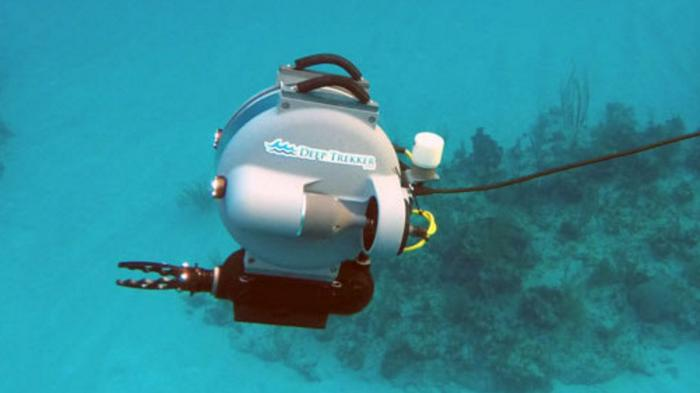
\includegraphics[width=6cm,height=5cm]{img/cap1/submarino1}}
    \subfigure[Robot OpenROV]{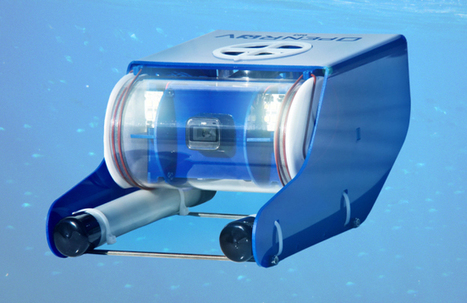
\includegraphics[width=6cm,height=5cm]{img/cap1/submarino2}}
  \end{center}
  \caption{Robots submarinos}
  \label{fig:submarino}
\end{figure}
  
\section{ROS}
\label{cap:ROS}

Sistema Operativo Robótico (en inglés \textit{Robot Operating System, ROS}\cite{ros}) es un framework para el desarrollo de software para robots que provee la funcionalidad de un sistema operativo en un clúster heterogéneo. 

Implementaremos ROS en el robot submarino ya que es el framework por excelencia para el desarrollo de las aplicaciones robóticas. Contiene algoritmos implementados, además de proporcionar una arquitectura distribuida. No hace falta que los nodos de ROS interactuen en el mismo sistema ni que deban ser de la misma arquitectura, por eso es una gran ventaja utilizarlo en la tecnología de OpenROV. 

ROS provee los servicios estándar de un sistema operativo tales como abstracción del hardware, control de dispositivos de bajo nivel, implementación de funcionalidad de uso común, paso de mensajes entre procesos y mantenimiento de paquetes. Está basado en una arquitectura de grafos donde el procesamiento toma lugar en los nodos que pueden recibir, mandar y multiplexar mensajes de sensores, control, estados, planificaciones y actuadores, entre otros.

ROS tiene dos partes básicas: la parte del sistema operativo, ROS, y una suite de paquetes aportados por la contribución de usuarios que implementan la funcionalidad, como localización y mapeo simultáneo, planificación, percepción, simulación, etc.

ROS es OpenSource bajo términos de licencia BSD. Esta licencia permite libertad para uso comercial e investigador.

\section{Estado del Arte}
\label{cap:Estado del Arte}
En base al estudio del estado del arte\cite{telemetria}, se establecen las variables necesarias para la manipulación del robot:
  \begin{itemize}
  \item \textbf{Aceleraciones en X, Y, Z} Obtiene el ángulo con respecto al plano. Por odometría se puede obtener la velocidad y la posición.
  \item \textbf{Velocidad angular en p, q y r (roll, pitch y yaw)} Por odometría, permite estimar perturbaciones en la rotación del robot.
  \item \textbf{Velocidades Lineales} Por odometría, se puede utilizar para compensar los errores acumulativos.
  \item \textbf{Presión Relativa} Permite conocer la profundidad a la que se ha sumergido.
  \item \textbf{Carga de Baterías} Permite conocer el estado de carga de las baterías. En caso de estar en un nivel crítico, se ejecutan modos de bajo consumo o de recuperación de la plataforma.
  \end{itemize}

\section{Estructura de la memoria}
\label{cap:estructuradelamemoria}
En este documento se describen los aspectos más relevantes del desarrollo y montaje del robot. La memoria esta dividida en 6 capítulos. 
El primer capítulo, Introducción, se ha realizado una presentación de los robots móviles. En el segundo capítulo se define el problema y se establecen los objetivos. El montaje del robot, el entorno y las herramientas utilizadas se especifica en el tercer capítulo. En el siguiente capítulo, el cuarto, se mostrará la integración del OpenROV con ROS. En el quinto capítulo se expondrán una serie de videos comprobando el funcionamiento del OpenROV, y en el último, el sexto, expondré las conclusiones del trabajo.
